\documentclass[letterpaper]{article} % DO NOT CHANGE THIS
\usepackage[submission]{aaai2027}  % DO NOT CHANGE THIS
% The serif, sans-serif, and monospaced fonts are loaded automatically by
% aaai2027.sty (newtxtext, helvet, courier). DO NOT add \usepackage{times},
% \usepackage{helvet}, \usepackage{courier}, or any other font package.
\usepackage[hyphens]{url}  % DO NOT CHANGE THIS
\usepackage{graphicx} % DO NOT CHANGE THIS
\urlstyle{rm} % DO NOT CHANGE THIS
\def\UrlFont{\rm}  % DO NOT CHANGE THIS
\usepackage{natbib}  % DO NOT CHANGE THIS AND DO NOT ADD ANY OPTIONS TO IT
\usepackage{caption} % DO NOT CHANGE THIS AND DO NOT ADD ANY OPTIONS TO IT
\frenchspacing  % DO NOT CHANGE THIS
%
% These are recommended to typeset algorithms but not required. See the subsubsection on algorithms. Remove them if you don't have algorithms in your paper.
\usepackage{algorithm}
\usepackage{algorithmic}

%
% These are recommended to typeset listings but not required. See the subsubsection on listing. Remove this block if you don't have listings in your paper.
\usepackage{newfloat}
\usepackage{listings}
\DeclareCaptionStyle{ruled}{labelfont=normalfont,labelsep=colon,strut=off} % DO NOT CHANGE THIS
\lstset{%
	basicstyle={\footnotesize\ttfamily},% footnotesize acceptable for monospace
	numbers=left,numberstyle=\footnotesize,xleftmargin=2em,% show line numbers, remove this entire line if you don't want the numbers.
	aboveskip=0pt,belowskip=0pt,%
	showstringspaces=false,tabsize=2,breaklines=true}
\floatstyle{ruled}
\newfloat{listing}{tb}{lst}{}
\floatname{listing}{Listing}

%
% Recommended for better-looking tables
\usepackage{booktabs}

%
% Keep the \pdfinfo as shown here. There's no need
% for you to add the /Title and /Author tags.
\pdfinfo{
/TemplateVersion (2027.1)
}

% DISALLOWED PACKAGES
% \usepackage{authblk} -- This package is specifically forbidden
% \usepackage{balance} -- This package is specifically forbidden
% \usepackage{CJK} -- This package is specifically forbidden
% \usepackage{float} -- This package is specifically forbidden
% \usepackage{flushend} -- This package is specifically forbidden
% \usepackage{fullpage} -- This package is specifically forbidden
% \usepackage{geometry} -- This package is specifically forbidden
% \usepackage{hyperref} -- This package is specifically forbidden
% \usepackage{navigator} -- This package is specifically forbidden
% (or any other package that embeds links such as navigator or hyperref)
% \usepackage{indentfirst} -- This package is specifically forbidden
% \usepackage{layout} -- This package is specifically forbidden
% \usepackage{multicol} -- This package is specifically forbidden
% \usepackage{nameref} -- This package is specifically forbidden
% \usepackage{savetrees} -- This package is specifically forbidden
% \usepackage{setspace} -- This package is specifically forbidden
% \usepackage{stfloats} -- This package is specifically forbidden
% \usepackage{tabu} -- This package is specifically forbidden
% \usepackage{titlesec} -- This package is specifically forbidden
% \usepackage{tocbibind} -- This package is specifically forbidden
% \usepackage{ulem} -- This package is specifically forbidden
% \usepackage{wrapfig} -- This package is specifically forbidden
% DISALLOWED COMMANDS
% \nocopyright -- Your paper will not be published if you use this command
% \addtolength -- This command may not be used
% \balance -- This command may not be used
% \baselinestretch -- Your paper will not be published if you use this command
% \clearpage -- No page breaks of any kind may be used for the final version of your paper
% \columnsep -- This command may not be used
% \newpage -- No page breaks of any kind may be used for the final version of your paper
% \pagebreak -- No page breaks of any kind may be used for the final version of your paper
% \pagestyle -- This command may not be used
% \tiny -- This is not an acceptable font size.
% \vspace{- -- No negative value may be used in proximity of a caption, figure, table, section, subsection, subsubsection, or reference
% \vskip{- -- No negative value may be used to alter spacing above or below a caption, figure, table, section, subsection, subsubsection, or reference

\setcounter{secnumdepth}{0} %May be changed to 1 or 2 if section numbers are desired.

% The file aaai2027.sty is the style file for AAAI Press
% proceedings, working notes, and technical reports.
%

% Title

% Your title must be in mixed case, not sentence case.
% That means all verbs (including short verbs like be, is, using,and go),
% nouns, adverbs, adjectives should be capitalized, including both words in hyphenated terms, while
% articles, conjunctions, and prepositions are lower case unless they
% directly follow a colon or long dash
\title{RC-GRPO: Reconstruction-Calibrated Temporal Credit Assignment for Tokenized Video World Models}
\author{Anonymous Submission}
\affiliations{}

%Example, Single Author, ->> remove \iffalse,\fi and place them surrounding AAAI title to use it
\iffalse
\title{My Publication Title --- Single Author}
\author {
    Author Name
}
\affiliations{
    Affiliation\\
    Affiliation Line 2\\
    name@example.com
}
\fi

\iffalse
%Example, Multiple Authors, ->> remove \iffalse,\fi and place them surrounding AAAI title to use it
\title{My Publication Title --- Multiple Authors}
\author {
    % Authors
    First Author Name\textsuperscript{\rm 1,\rm 2}\equalcontrib,
    Second Author Name\textsuperscript{\rm 2}\equalcontrib,
    Third Author Name\textsuperscript{\rm 1}\corresponding
}
\affiliations {
    % Affiliations
    \textsuperscript{\rm 1}Affiliation 1\\
    \textsuperscript{\rm 2}Affiliation 2\\
    firstAuthor@affiliation1.com, secondAuthor@affilation2.com, thirdAuthor@affiliation1.com
}
\fi


\begin{document}

\maketitle

\begin{abstract}
Action-conditioned video world models provide learned dynamics for robotic planning, interactive simulation, and model-based decision making. Recent verifiable-reward post-training samples candidate futures, decodes them, and applies GRPO using full-reference errors to ground-truth frames. Yet a computable verifier need not be a reliable learning signal. Frozen visual tokenizers confine candidates to a codec-reachable set, whereas raw targets are generally not exactly reproducible; candidate-dependent interactions with the target reconstruction residual can change the within-group ordering consumed by GRPO. Multi-step training further broadcasts one sequence-level advantage across future-frame visual-token blocks with different downstream influence. We introduce RC-GRPO, which audits raw-versus-reachable rank disagreement, scores candidates against tokenizer reconstructions, anchors calibrated updates to first-order progress under the raw verifier, and assigns each future-frame token block the return of subsequent frames it can affect. Reconstruction audits show non-negligible encode--decode reconstruction errors for three independently designed FSQ codec instances, including NVIDIA Cosmos DV-FSQ, while same-candidate audits on RT-1 and VP2-RoboSuite show improved agreement with decoder-input representation error and fewer pairwise rank flips across tokenizers and generative architectures. On RT-1 episodes excluded from training, temporal return improves the mean of all five fidelity metrics over sequence-level calibration: MSE improves in all five paired seeds and the remaining metrics in four of five, although paired $t$ tests remain below conventional significance. The evidence supports calibrating both comparison support and temporal credit, but does not establish universal raw-pixel gains across platforms or improvements in motion and distributional realism.
\end{abstract}

% Uncomment the following to link to your code, datasets, an extended version or similar.
% You must keep this block between (not within) the abstract and the main body of the paper.
% Make sure that you do not de-anonymize yourself with these links.
% \begin{links}
%     \link{Code}{https://aaai.org/example/code}
%     \link{Datasets}{https://aaai.org/example/datasets}
%     \link{Extended version}{https://aaai.org/example/extended-version}
% \end{links}

\section{Introduction}

Video world models predict action-conditioned future observations and thereby provide sampleable dynamics for robotic planning, interactive simulation, and model-based reinforcement learning \citep{worldmodels,rssm,dreamerv3,dws}. Tokenized implementations make high-dimensional video prediction tractable by encoding frames into discrete visual tokens, modeling future tokens autoregressively, and decoding them back to images \citep{videogpt,magvit,ivideogpt,fsq}. Verifiable-reward post-training offers a complementary route to improvement: for each context and action sequence, it samples a group of candidate futures, scores their decoded frames against observed futures, and applies GRPO to reinforce candidates with higher within-group rewards \citep{rlvrworld,grpo}. This is especially attractive for world models because the supervision is externally computable and directly tied to prediction fidelity.

Existing research has progressed along three largely separate directions. World-model and tokenizer work improves the generative backbone or the visual representation \citep{vqvae,vqgan,fsq}; verifier design selects decoded full-reference metrics such as MSE, SSIM, and LPIPS \citep{ssim,lpips}; and GRPO variants refine the optimization objective or assign finer credit to reasoning and generative trajectories \citep{grpolambda,spo,sdgrpo,stepwiseflowgrpo,dapo}. None of these directions resolves two mismatches created when a frozen visual tokenizer is placed inside a group-relative video post-training loop. First, every decoded candidate belongs to the decoder-reachable set, whereas a raw ground-truth frame is generally not exactly reproducible by the same tokenizer. Group centering removes the candidate-independent part of this reconstruction residual, but not its interaction with candidate errors; that interaction can reverse the pairwise ordering that GRPO actually consumes. The problem is therefore not merely a large reconstruction error or a missing image metric, but an unreliable relative preference on the policy's feasible outputs. Second, multi-step video GRPO commonly broadcasts one sequence-level advantage to all future-frame token blocks. This ignores their asymmetric downstream influence, while independent frame-level advantages are myopic because they sever credit from later frames that depend on earlier generations.

To address both mismatches, we introduce \emph{RC-GRPO} while leaving candidate sampling, the frozen visual tokenizer, the decoder, and raw-frame evaluation unchanged. On the verifier side, a \emph{Reachability Audit} rescoring the same candidate group against the raw frame and its tokenizer reconstruction measures rank correlation and pairwise preference flips before training. The reconstruction-calibrated verifier then retains the original MSE and LPIPS but compares candidates with the reachable reconstruction $\tilde{s}'_h=D(Q(E(s'_h)))$. Because replacing the target can alter progress toward raw ground truth, a raw-anchored update constructs raw and calibrated group-relative surrogates on the same candidates and projects the calibrated direction onto a half-space that preserves first-order progress under the raw surrogate. On the temporal side, the $t$-th future-frame token block receives the return of frame rewards from $t$ to the end of the rollout, normalized only across candidates at the same temporal position. RC-GRPO thus forms one chain of reachable-set comparison, raw-fidelity-constrained updating, and autoregressive block-level credit, rather than appending more image metrics to a generic GRPO variant.

Our contributions are twofold. First, we identify target-set mismatch as a candidate-ranking failure in tokenized video post-training and develop reachability-constrained rank calibration, comprising a pre-training audit, a reconstruction-calibrated verifier, and a raw-anchored update. Reconstruction audits establish non-negligible encode--decode reconstruction errors for CNN-FSQ, compressive FSQ, and the independently designed Cosmos DV-FSQ codec; same-candidate audits on RT-1 and VP2-RoboSuite further show improved agreement with decoder-input representation error and fewer pairwise flips across different tokenizers and generative architectures. All final fidelity metrics remain evaluated against raw ground truth. These audits establish the cross-codec reconstruction mismatch and cross-world-model ranking mechanism, not a universal raw-pixel training gain. Second, we introduce frame-block temporal-return credit assignment for autoregressive video rollouts, changing the credit unit from an entire sequence to the future-frame token block and returning later visual quality only to blocks that can influence it. Under an episode-disjoint RT-1 evaluation, temporal return improves all five mean fidelity metrics over sequence-level calibration; MSE improves in 5/5 paired seeds and LPIPS, LPIPS-last, PSNR, and SSIM in 4/5. Our claims are limited to directional full-reference evidence and do not imply universal improvements in motion fidelity or distributional realism.

\section{Related Work}

\paragraph{Tokenized video world models.}
World models learn predictive environment dynamics that can support planning, control, and simulation from visual observations \citep{worldmodels,rssm,dreamerv2,dreamerv3}. Recent video generative models extend this idea by modeling future visual observations directly, often through tokenized sequence modeling. VideoGPT, MAGVIT, iVideoGPT, Genie, and pre-trained video simulators show that discrete visual tokens and autoregressive or masked sequence models can support scalable video prediction and interactive generation \citep{videogpt,magvit,ivideogpt,genie,dws}. These works mainly study how to build or pre-train a sampleable video world model. Our focus is different: given a tokenized video world model and a verifiable post-training loop, we study whether the decoded verifier target and the sequence-level GRPO update match the structure of tokenized multi-step video prediction.

\paragraph{Verifiable reward post-training.}
Verifiable reward training samples multiple candidate outputs for the same context, scores them with an externally computable reward, and applies group-relative policy updates without a learned value function. RLVR-World instantiates this idea for world models, while GRPO and related RLVR-style methods have been widely explored in language reasoning and post-training \citep{rlvrworld,grpo,deepseekr1}. Recent variants change normalization, clipping, importance ratios, or sample selection. We do not treat generic optimizer variants as direct solutions to tokenized video post-training. In our setting, the verifier itself can alter within-group rankings because decoded candidates are compared with targets that are not exactly reachable through the tokenizer-decoder pair. This shifts the relevant intervention from an optimizer swap to video-structured verifier calibration.

\paragraph{Visual tokenizers and evaluation metrics.}
Discrete visual representation learning compresses images or videos into token sequences that can be modeled by transformers, but lossy tokenization introduces an encode-decode reconstruction limit \citep{vqvae,vqgan,fsq}. This limit is closely related to the broader perception-distortion tradeoff in image reconstruction \citep{perceptiondistortion}. Full-reference metrics such as SSIM and LPIPS are commonly used to evaluate per-sample fidelity, whereas FID, KID, FVD, DINO-based distances, precision/recall, and density/coverage evaluate distribution-level fidelity and diversity \citep{ssim,lpips,fid,kid,fvd,dinov2,precisionrecall,densitycoverage}. These metrics are usually used for reporting generation quality. We instead ask what happens when a post-decode full-reference metric becomes the reward consumed by GRPO: distribution-level metrics do not directly provide a per-candidate verifier, while post-decode per-sample metrics inherit the tokenizer reconstruction residual and can alter candidate rankings.

\paragraph{Fine-grained credit assignment.}
Sequence-level advantages can be too coarse when a generation trajectory contains multiple decisions or generation stages. Classical return-based credit assignment and recent step-level post-training methods both distinguish delayed outcomes from immediate rewards. RC-GRPO applies this principle to tokenized autoregressive video rather than claiming reward-to-go as a new construction. Here the credit unit is a future-frame block of visual tokens, each decoded into a state prediction that can be scored against its observed future frame. This motivates temporal-return advantages over frame blocks rather than one task-agnostic rollout scalar.

\section{Preliminaries}

\paragraph{Problem setup.}
We study verifiable post-training for action-conditioned tokenized video world models. Given a context $q_t$ consisting of past observations and actions, the model predicts future visual states $s_{t+1:t+H}$. A visual tokenizer $E$ maps each frame to discrete visual tokens, and a decoder $D$ maps generated tokens back to image space. We write the world model as an autoregressive policy $\pi_\theta$ over future visual tokens conditioned on $q_t$ and previously generated tokens. This paper does not modify the tokenizer, decoder, or backbone world model; it studies whether the verifier target and the GRPO update are aligned with this tokenized generation interface.

\paragraph{Verifiable reward training.}
In an RLVR-style update, the policy samples a group of $G$ candidate futures for the same context. Each candidate token sequence is decoded into a visual prediction $\hat{s}_i$, and a verifier assigns a reward $R_i$ by comparing the prediction with a target frame. GRPO normalizes rewards within the sample group,
\begin{equation}
A_i=\frac{R_i-\mu_R}{\sigma_R+\epsilon},
\label{eq:groupnorm}
\end{equation}
and uses $A_i$ to weight the log-probability of the sampled tokens. Because the normalization is group-relative, the effective training signal is not the absolute reward value alone, but the relative ordering and spacing of candidates within the group.

\paragraph{Multi-step rollouts.}
Single-step prediction evaluates one future frame. In a multi-step rollout, the model generates a sequence of future-frame token blocks, and decoded early frames become part of the context for later predictions. Let $r_{i,u}$ denote the frame-level reward of candidate $i$ at future horizon $u$; following the multi-step reward convention of RLVR-World \citep{rlvrworld}, the first future frame carries no direct action-conditioned reward, so $r_{i,1}=0$. A standard sequence-level GRPO baseline aggregates frame rewards into one rollout-level scalar,
\begin{equation}
R_i^{\mathrm{seq}}=\frac{1}{H-1}\sum_{u=2}^{H}r_{i,u},
\label{eq:seqreward}
\end{equation}
and broadcasts the resulting advantage to all generated tokens in the rollout. This defines the credit-assignment problem studied in this paper: tokenized video prediction is autoregressive across future frames, but a single sequence-level advantage cannot distinguish the responsibility of different future-frame token blocks.

\section{Method}

% ------------------------------------------------------------------
% RESERVED: Figure (overall architecture / pipeline).
% Planned content: tokenized world-model RLVR loop with the two RC-GRPO
% intervention points highlighted — (1) verifier target s_t -> D(E(s_t)),
% (2) rollout-scalar advantage -> per-horizon temporal-return advantages
% on future-frame token blocks. Suggested placement: figure* at top of
% the Method page. Uncomment when Figures/fig_pipeline.pdf is ready.
% \begin{figure*}[t]
% \centering
% \includegraphics[width=0.95\textwidth]{Figures/fig_pipeline.pdf}
% \caption{RC-GRPO overview. A tokenized video world model samples a group
% of candidate rollouts; RC-GRPO changes exactly two points of the training
% signal: the verifier compares decoded frames with the tokenizer-reachable
% target $\tilde{s}_t=D(E(s_t))$, and each future-frame token block receives
% a per-horizon, group-normalized temporal-return advantage instead of one
% broadcast sequence-level scalar.}
% \label{fig:pipeline}
% \end{figure*}
% ------------------------------------------------------------------

\paragraph{Overview.}
RC-GRPO keeps the RLVR-style sample group, verifiable metric, and world-model architecture intact, but changes how the training signal is constructed. It audits and calibrates the verifier target to the frozen codec's reachable set, anchors the calibrated gradient to first-order progress under the raw verifier, and assigns multi-step advantages to future-frame token blocks through temporal returns rather than broadcasting one rollout-level scalar.

\paragraph{Reconstruction-calibrated verifier.}
For a full-reference distance $d$, a lossy tokenizer induces an encode--decode reconstruction residual
\begin{equation}
\phi_{\mathrm{tok}}^{(d)}
=
\mathrm{E}_{s_t}
\left[d(D(E(s_t)),s_t)\right].
\end{equation}
This term is not caused by a sampled candidate, but it is included when a post-decode verifier compares a decoded prediction with the raw frame. For a candidate group, let $\delta_i=r_i^{\mathrm{raw}}-r_i^{\mathrm{reach}}$, $c=G^{-1}\sum_i\delta_i$, and $\eta_i=\delta_i-c$. Then $r_i^{\mathrm{raw}}=r_i^{\mathrm{reach}}+c+\eta_i$. Group centering removes $c$, but not the candidate-dependent $\eta_i$; the latter can therefore change within-group ranks and spacings. RC-GRPO removes this target mismatch by replacing the raw target $s_t$ with the tokenizer-reachable target
\begin{equation}
\tilde{s}_t = D(Q(E(s_t))).
\end{equation}
Given a decoded prediction $\hat{s}_{i,t}$, the reconstruction-calibrated reward is
\begin{equation}
r_{i,t}^{\mathrm{RC}}
=
-d(\hat{s}_{i,t},\tilde{s}_t).
\end{equation}
In our multi-step experiments we instantiate $d$ with the RLVR-World full-reference evaluator,
\begin{equation}
r_{i,t}^{\mathrm{RC}}
=
-\left[
\mathrm{MSE}(\hat{s}_{i,t},\tilde{s}_t)
+
\mathrm{LPIPS}(\hat{s}_{i,t},\tilde{s}_t)
\right].
\end{equation}
The raw verifier used for comparison replaces $\tilde{s}_t$ with $s_t$. The target remains verifiable because $\tilde{s}_t$ is deterministically obtained from the ground-truth frame and the frozen tokenizer; the change is that reward construction compares candidates in the image space reachable by the tokenizer--decoder pair. Final evaluation remains against the raw frame $s_t$, so the calibrated target cannot improve a reported metric by definition alone.

\paragraph{Raw-anchored calibrated update.}
Replacing the target can improve reachable-space ordering without guaranteeing finite-step progress on raw-frame fidelity. We therefore construct raw and calibrated GRPO surrogate losses on the same candidates and with the same credit mode. Let $g_0=\nabla_\theta\ell_{\mathrm{raw}}$ and $g_1=\nabla_\theta\ell_{\mathrm{RC}}$. We choose the direction closest to $g_1$ whose first-order raw-surrogate progress is at least that of the raw update:
\begin{equation}
g^*=\arg\min_g\frac{1}{2}\|g-g_1\|_2^2
\quad\mathrm{s.t.}\quad
\langle g,g_0\rangle\geq\|g_0\|_2^2.
\end{equation}
The half-space projection has the closed form
\begin{equation}
g^*=g_1+\lambda^*g_0,\qquad
\lambda^*=\frac{[\|g_0\|_2^2-\langle g_1,g_0\rangle]_+}
{\|g_0\|_2^2+\epsilon}.
\end{equation}
This is a sampled-surrogate, first-order constraint rather than a guarantee on held-out raw LPIPS. The reference-policy regularizer is added once after the projection.

\paragraph{Temporal-return GRPO.}
Let a candidate rollout contain $H$ future-frame token blocks $o_{i,t,1:N}$, where $N$ is the number of visual tokens per frame block. Standard sequence-level GRPO assigns the group-normalized advantage of the rollout-level scalar $R_i^{\mathrm{seq}}$ in Eq.~\ref{eq:seqreward} to every generated token. RC-GRPO instead computes a temporal return for each future-frame block,
\begin{equation}
G_{i,t}
=
\sum_{u=t}^{H}
\beta^{u-t} r_{i,u}^{\mathrm{RC}},
\end{equation}
where $\beta$ is a temporal discount. The first future frame has no direct reward ($r_{i,1}=0$, as in the preliminaries), but it can still receive credit through later rewards in $G_{i,1}$. For each horizon $t$, we normalize returns across the candidates in the same sample group:
\begin{equation}
A_{i,t}^{\mathrm{return}}
=
\frac{G_{i,t}-\mu_t}{\sigma_t+\epsilon},
\end{equation}
where $\mu_t$ and $\sigma_t$ are computed over $\{G_{i,t}\}_{i=1}^{G}$.

\paragraph{Optimization.}
The temporal-return advantage weights the log-probability of the corresponding future-frame token block. Let
\begin{equation}
\ell_{i,t}
=
\sum_{\tau=1}^{N}
\log
\pi_{\theta}
\left(o_{i,t,\tau}\mid h_{i,t,\tau}\right),
\end{equation}
where $h_{i,t,\tau}$ denotes the autoregressive context of token $\tau$ in block $t$: the window context, the injected actions, and all previously generated tokens. The policy-gradient loss is
\begin{equation}
\mathcal{L}_{\mathrm{RCG}}
=
-\frac{1}{G}
\sum_{i=1}^{G}
\sum_{t=1}^{H}
A_{i,t}^{\mathrm{return}}\ell_{i,t}.
\end{equation}
If $A_{i,t}^{\mathrm{return}}$ is replaced by the same sequence-level advantage for all $t$, the objective reduces to the sequence-level GRPO baseline. In implementation, multi-step training also uses a small reference-policy anchor,
\begin{equation}
\mathcal{L}
=
\mathcal{L}_{\mathrm{RCG}}
+
\lambda_{\mathrm{KL}}
\widehat{D}_{\mathrm{KL}}
\left(\pi_\theta\|\pi_{\mathrm{ref}}\right),
\end{equation}
where $\pi_{\mathrm{ref}}$ is the frozen base world model. Following the official video recipe, we use the sampled low-variance form $\exp(k)-k-1$ with $k=\log\pi_{\mathrm{ref}}-\log\pi_\theta$. Each sampled group is consumed by exactly one gradient step. The anchor is applied consistently across multi-step arms to reduce policy drift; horizon-aware variants and gain-shaped rewards are not part of the method.

\section{Experiments}

\paragraph{Experimental setup.}
We evaluated RC-GRPO on the RT-1 \texttt{fractal20220817} action-conditioned video data \citep{rt1} using the public RLVR-World multi-step base checkpoint and its fixed visual tokenizer \citep{rlvrworld}. Training uses 24 fixed windows, one context frame, and seven future frames. Formal evaluation uses all 32 stride-8 windows from eight episodes absent from training. Each update samples $G=16$ rollouts with temperature $1.0$ and top-$k=100$. All formal multi-step runs use 30 updates, learning rate $10^{-5}$, two windows per update, temporal discount $\beta=0.95$, and the official sampled low-variance KL with coefficient $0.001$. Every arm uses paired seeds 0--4 and the fixed final checkpoint. All metrics compare predictions with raw future frames, never reconstructed targets. We additionally audit frozen candidate groups on VP2-RoboSuite to test whether rank calibration transfers across tokenizers and generative architectures, and use NVIDIA Cosmos DV-FSQ \citep{nvidia2025cosmoswfm} as an independent codec reconstruction-floor audit without making a candidate-ranking claim for Cosmos.

\begin{figure}[t]
\centering
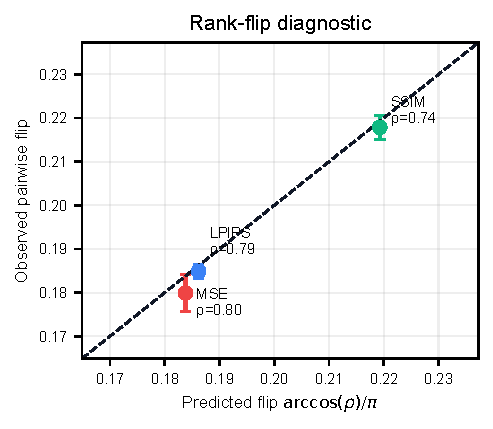
\includegraphics[width=\columnwidth]{Figures/fig_rank_flip.pdf}
\caption{Rank-disagreement diagnostic for decoded verifiers. Across five generation repetitions, the observed pairwise disagreement with a pre-decode code-space reference closely follows the predicted $\arccos(\rho)/\pi$ rate. The code-space score is used as a residual-free diagnostic reference, not asserted to be the uniquely correct reward.}
\label{fig:rank_flip}
\end{figure}

\paragraph{Rank disagreements match the verifier-noise prediction.}
Before evaluating training outcomes, we tested whether reconstruction-induced reward variation changes the within-group ordering consumed by GRPO. For each candidate group, we correlate a decoded reward with a pre-decode code-space score of the same candidates and denote the correlation by $\rho$. The pre-decode score is not treated as ground-truth quality; it is a diagnostic reference that does not pass through the decoder. Under a jointly Gaussian score model, the probability that a candidate pair is ordered differently is the bivariate-Gaussian orthant probability $\arccos(\rho)/\pi$. Figure~\ref{fig:rank_flip} shows that this prediction tracks observed pairwise disagreement for LPIPS, MSE, and SSIM. We then rescore identical groups with RC. Across 184 held-out contexts and five independently sampled candidate groups per context (920 groups in total), aggregate disagreement decreases for LPIPS ($0.162\rightarrow0.151$), MSE ($0.181\rightarrow0.168$), and MSE+LPIPS ($0.160\rightarrow0.149$); all five generation repetitions show the same decrease, and the prediction remains within $0.005$ of the observed rate before and after calibration. Because contexts repeat across generation runs, we treat these values as a five-repetition diagnostic rather than 920 independent trials. Together, the results show that reachable-target calibration reduces measured rank disagreement; they do not claim that the code-space ordering is uniquely correct.

\begin{table*}[t]
\centering
\caption{Episode-disjoint multi-step comparison using the sampled low-variance KL objective. Trained rows report means over paired seeds 0--4 at the fixed final checkpoint on 32 windows from eight episodes absent from training. The public RLVR-World checkpoint is evaluation-only.}
\label{tab:main_multistep}
\small
\setlength{\tabcolsep}{4pt}
\begin{tabular}{lcccccc}
\toprule
Method & Seeds & LPIPS $\downarrow$ & LPIPS-last $\downarrow$ & MSE $\downarrow$ & PSNR $\uparrow$ & SSIM $\uparrow$ \\
 \midrule
Base world model & eval-only & 0.21273 & 0.22783 & 0.015480 & 18.827 & 0.73749 \\
RLVR-World checkpoint & eval-only & 0.20403 & 0.21206 & 0.014390 & 19.106 & 0.75323 \\
Seq-GRPO, raw verifier & 0--4 & 0.19915 & 0.21180 & 0.013679 & 19.403 & 0.75555 \\
\midrule
Seq-GRPO, RC verifier (\emph{Ours}) & 0--4 & 0.19933 & 0.21176 & 0.013820 & 19.382 & 0.75577 \\
Temporal return, raw verifier & 0--4 & 0.20118 & 0.21487 & 0.013941 & 19.341 & 0.75362 \\
Temporal return, RC verifier (\emph{Ours}) & 0--4 & $\mathbf{0.19657}$ & $\mathbf{0.20767}$ & $\mathbf{0.013556}$ & $\mathbf{19.447}$ & $\mathbf{0.75908}$ \\
\midrule
$\Delta$ vs. sequence RC & -- & $\mathbf{-1.39\%}$ & $\mathbf{-1.93\%}$ & $\mathbf{-1.91\%}$ & $\mathbf{+0.33\%}$ & $\mathbf{+0.44\%}$ \\
\bottomrule
\end{tabular}
\end{table*}

\paragraph{Main results.}
Table~\ref{tab:main_multistep} reports the formal episode-disjoint factorial. Temporal return with the RC verifier attains the best mean on all five metrics. Relative to sequence-level RC, it reduces LPIPS by $0.002764$ (4/5 paired seeds, $t=-1.94$, two-sided $p=0.125$), LPIPS-last by $0.004093$ (4/5, $t=-1.79$, $p=0.149$), and MSE by $0.000264$ (5/5, $t=-2.40$, $p=0.074$), while improving PSNR and SSIM in 4/5 seeds. The exact one-sided sign-flip test for MSE is $p=0.031$, but none of the paired $t$ tests reaches two-sided $0.05$. The four-arm LPIPS interaction is also nonsignificant ($p=0.309$), so the lowest full-stack mean is not evidence of statistical super-additivity.

\paragraph{Cross-codec reconstruction residual and cross-world-model rank audits.}
We next test the C1 mechanism without assuming that an improved diagnostic must already translate into raw-pixel gains after policy optimization. Under the same LPIPS-VGG readout, the encode--decode reconstruction residual is approximately $0.053$ for CNN-FSQ, $0.077$ for compressive FSQ, and $0.190$ for the independently designed NVIDIA Cosmos DV-FSQ video codec. These values establish non-negligible reconstruction residuals across three FSQ codec instances; because their resolutions and temporal compression protocols differ, we do not interpret the magnitudes as a controlled monotonic compression law. On VP2-RoboSuite, where matched candidate groups are available, RC increases same-candidate Spearman agreement by $0.0932$ at horizon 2 and by $0.0753$ at horizon 8, while reducing pairwise disagreement by $0.0409$ and $0.0346$, respectively. The bootstrap confidence intervals exclude zero. Thus the reconstruction audit and the rank audit play distinct roles: Cosmos tests whether the target mismatch recurs in an independent codec, whereas VP2 tests whether reachable-target calibration repairs candidate ordering in another world-model pipeline.

\paragraph{Evidence boundary and pending controls.}
The cross-platform result above establishes rank repair, not universal improvement under a raw-ground-truth evaluation target. A three-seed RT-1 pilot supports the proposed raw-anchored update, whereas VP2 has not shown a reliable raw-pixel training gain; Cosmos has no matched policy-training experiment. We therefore keep cross-platform policy improvement outside the present claim. For temporal credit, the formal result is the paired five-seed comparison in Table~\ref{tab:main_multistep}; sequence, framewise, return, and shuffled-return controls under the same low-variance-KL objective remain the required test for attributing the gain specifically to future-return structure. We likewise make no claim about motion quality or distributional realism from the current full-reference results.

\section{Conclusion}

Post-decode verifiers and sequence-level advantages each overlook structure in tokenized video: the raw target need not lie in the frozen codec's reachable image set, and one sequence-level advantage cannot distinguish the responsibility of autoregressive future-frame blocks. RC-GRPO modifies these two interfaces. Non-negligible encode--decode reconstruction errors across CNN-FSQ, compressive FSQ, and Cosmos DV-FSQ show that target mismatch is not confined to one project tokenizer; reachable-target calibration then reduces same-candidate rank disagreement on RT-1 and VP2-RoboSuite, while the raw-anchored update preserves the original evaluation direction when the two verifier gradients disagree. Temporal-return credit achieves the best mean RT-1 fidelity on training-disjoint episodes, with MSE improving in all five paired seeds and the remaining metrics in four. Cross-platform raw-pixel policy gains, conventional two-sided significance, and the full set of temporal-structure controls remain evidence boundaries. Within this scope, the results support aligning both verifier targets and credit units with the tokenized video generation process.

\paragraph{Data and code availability.}
We use the publicly available RT-1 data cited above. Processed source data for all manuscript figures are included with the submission, together with analysis scripts and the configurations needed to reproduce the reported tables. Training code and model-output summaries are provided in the anonymous supplementary archive.

\bibliography{aaai2027}

% Check whether the conference requires a reproducibility checklist to be included in the paper.
% If so, you can uncomment the following line and ajust the path to include it.
% \input{ReproducibilityChecklist.tex}

\end{document}
